% Autor: João Fiuza de Alencastro

\documentclass[journal]{IEEEtran}
\usepackage{listings}
\usepackage{verbatim}
\usepackage[utf8]{inputenc}
\usepackage{graphicx}
\usepackage{cite}
\usepackage[colorlinks=true,urlcolor=red,citecolor=blue,linkcolor=blue]{hyperref}
\RequirePackageWithOptions{multicol}



\begin{document}

\title{Sistemas de prevenção de intrusão\\ em ambientes de nuvem IoT}


\author{João~Fiuza~de~Alencastro\\Departamento~de~Engenharia~Elétrica\\Universidade~de~Brasília}% <-this % stops a space




% make the title area
\maketitle


\begin{abstract}
Pela sua natureza distribuída, ambientes \textit{'clusterizados'} são alvos fáceis de serem explorados. Atacantes disfarçados de usuários legítimos, por exemplo, podem se aproveitar dos abundantes recursos que a nuvem pode oferecer. Neste artigo é discutido como um sistema de detecção de intrusão distribuído em nuvem funciona inserido em um contexto de Internet das Coisas, assim também como suas vantagens e desvantagens.%   e possíveis melhorias na tecnologia existente.
\end{abstract}

\begin{IEEEkeywords}
Cloud computing, Intrusion Detection, Intrusion Prevention, security, IoT.
\end{IEEEkeywords}


\IEEEpeerreviewmaketitle



\section{Introdução}
\IEEEPARstart{A}{o} analisar ambientes em nuvem, deve-se ter sempre uma visão distribuída dos componentes da topologia. Assim como aplicações comuns da internet, esses ambientes também são alvos de ataques mal intencionados. \par
Os nós - que podem ser desde aplicações em sistemas finais a microprocessadores atuando como medidores - fazem parte dessa composição, esses quais devem ser monitorados individualmente, e quando um ataque ocorre, o tratamento dos dados provenientes desses sistemas deve ser tratado de forma diferente. Quais são as atitudes que podem ser tomadas em tais circunstâncias? A confiabilidade e integridade desses dados serão comprometidos para sempre? \par
O monitoramento pode ser realizado por sistemas de detecção de intrusão a nível de rede, porém toda a comunicação requer compatibilidade entre os diferentes hospedeiros, mecanismos de comunicação, e permissões de controle sobre manutenções e atualizações dos sistemas. Middlewares em nuvem normalmente provêm tais funcionalidades, portanto uma opção interessante seria um serviço de NIDS ("Network Intrusion Detection System") oferecido na camada de middleware (em oposição às camadas de infraestrutura e de software) $^{ [1] }$.

\section{Computação em Nuvem}
A computação em nuvem é um modelo computacional no qual os recursos são providos como um serviço através da internet. Movida conforme a demanda, ela trabalha desafogando do usuário a responsabilidade de comprar e gerenciar equipamentos complexos e dedicados de infraestrutura. \par
O aluguel de recursos computacionais sob-demanda desloca a responsabilidade de gerência e administração para uma equipe de especialistas, reduzindo os riscos de segurança tipicamente oriundos de má configuração de sistema, falta de atualizações, ou comportamento indevido do usuário. Apesar disso, o ambiente em nuvem introduz um risco considerável ao fazer com que os usuários compartilhem recursos físicos. \par
O sistema de computação em nuvem de interesse é voltado para Internet das Coisas (IoT), porém os princípios continuam os mesmos, assim como as vulnerabilidades. Na figura [1] abaixo, é possível verificar a topologia proposta. \par
Cada um desses riscos de segurança deve ser tratado de forma cautelosa e de forma específica, seja o ataque conhecido ou não, deve ser detectado e devidamente analisado. Esta é outra razão pela qual uma solução integrada, levando em conta diferentes aspectos relacionados à segurança é necessária para proteger dados de usuários e prevenir ações maliciosas contra ambientes em nuvem$^{ [2] }$.

% figura 1
\begin{figure}[h!]
	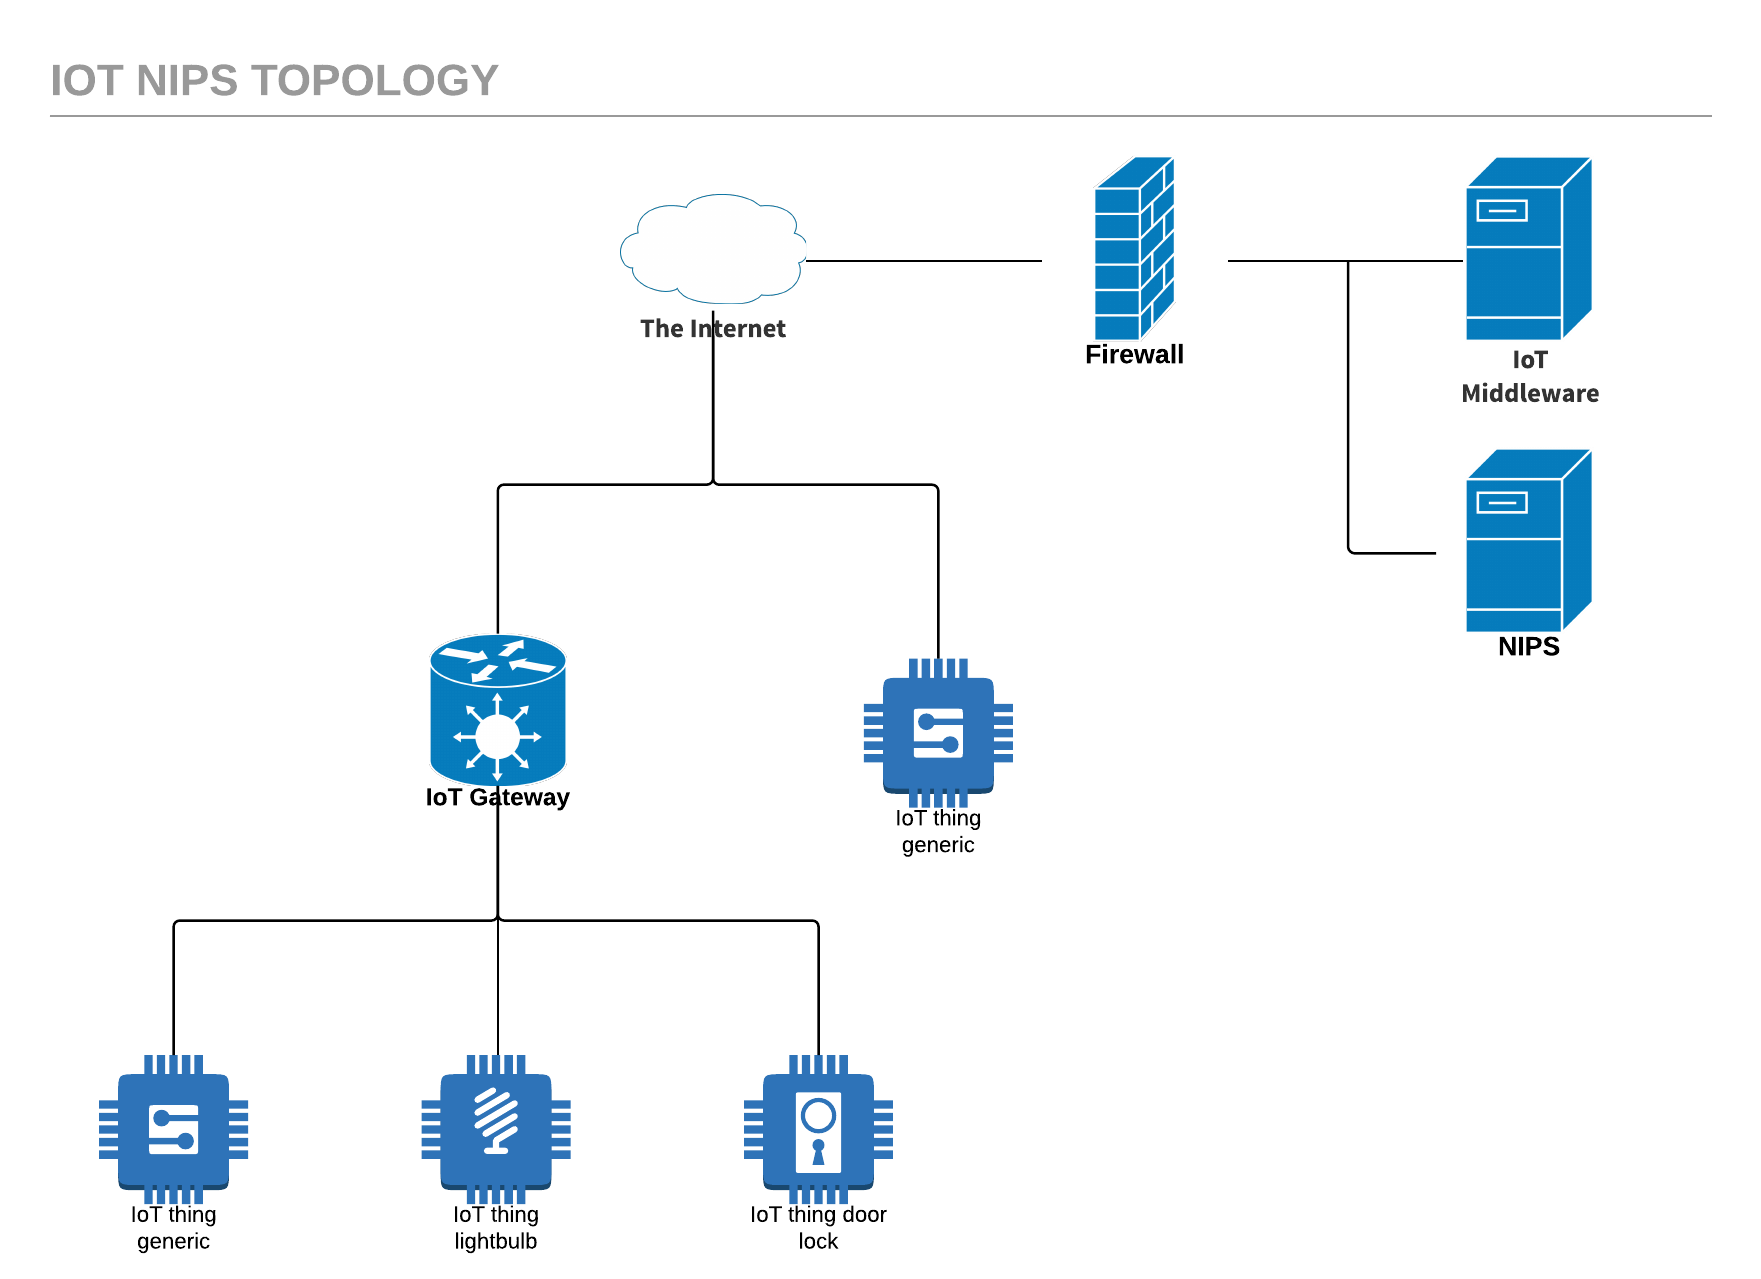
\includegraphics[width=\linewidth]{IoT_NIPS_topology_firewall.png}
	\caption{Topologia da instância IoT}
	\label{fig:NIPS_IoT_Topology}
\end{figure}

\section{Middleware}
Por que o sistema de detecção deve se encontrar a nível de middleware, como foi mencionado? Como o sistema de prevenção de intrusão proposto atua na camada de rede da pilha TCP/IP, ele deve ser capaz de "observar" todo o tráfego da rede, abstraindo a aplicação e focando seus poderes de processamento em ataques de rede, como o DDoS, por exemplo. Além disso, em um contexto com recursos escassos, como o de IoT, a camada de middleware permite uma disponibilidade maior para o processamento, retirando responsabilidades dos pequenos dispositivos que participam do serviço. E por fim, IDS a nivel de middleware apresenta facilidade de administração e orquestração dos componentes da topologia. Todos esses aspectos contribuem para o fato de o NIPS estar localizado a mesma rede local do middleware, compartilhando recursos de rede. \par
Os nós contêm os recursos, enquanto que o middleware define as políticas de acesso e controle e suporta um ambiente orientado a serviço. \par


\section{Intrusões em 'Grid'}
\subsection{Acesso não-autorizado}
É uma intrusão feita por alguém que não deveria ter acesso por meio de uma máscara ou um disfarce de usuário legítimo. Pode ser feito conseguindo a senha do usuário, seja por roubo, força bruta, palpitação, ou até mesmo por descuido do mesmo. Ataques ao serviço de autenticação é outra possibilidade, porém pode deixar rastros.
\subsection{Uso indevido}
Pode ser uma consequência de (A), configurado como abuso de privilégios de um usuário legítimo e geralmente resulta em um comportamento anômalo. Depende de quais políticas foram definidas pelo prestador do serviço.
\subsection{Ataque em 'Grid'}
Ataques realizados com a utilização de ferramentas ou scripts de \textit{'exploits'} que almejam vulnerabilidades de protocolos,serviços e aplicações em 'grid'. Esses podem aparecer em forma de negação de serviço, sondas, e vermes, e pdem deixar rastros de sua existência em vários pontos a infraestrutura.
\subsection{Instrusões específicas de hospedeiro/rede}
Enquanto que (A), (B) e (C) são ataques específicos em 'grid', estes são quaisquer outros ataques aos hospedeiros ou à rede$^{ [3] }$.

\section{Proposta IoT}
\subsection{Detecção de Intrusão}
Além da detecção de tentavas de intrusão no sistema, é preferível que haja algum tipo de ação, que o sistema tome atitudes em relação àquela atividade mal intencionada. Então, é introduzida a ideia de "Network Intrusion Prevention System" (NIPS), que age para que os ataques sejam impedidos. Neste caso em questão, a inteligência do sistema se encontra no middleware IoT, dessa forma, quando o NIPS precisar realizar alguma rotina de ação, ao invés disso, ele deverá se comunicar com o middleware, para que ele possa realizar essa ação. Esse processo é dado dessa forma para que as medidas não sejam tomadas de uma forma descentralizada, pois um ambiente de internet das coisas deve estar em sincronia com todos os seus componentes. \par
Em um primeiro momento, será utilizado somente a detecção de intrusos baseado em anomalias, ou seja, tráfegos suspeitos serão analisados, e possívelmente, bloqueados. A técnica de detecção por anomalias apresenta maior prevenção para o sistema, já que pode detectar ataques 'zero day', ou seja, ataques previamente desconhecidos.
\subsection{Comunicação}
A comunicação entre o NIPS e o middleware será feita através de uma API REST. Dessa forma, o NIPS poderá adicionar/retirar/modificar endereços no middleware. A ideia é implementar uma espécie de 'blacklist' no middleware, uma lista na qual o NIPS irá controlar através da comunicação com o middleware. Quando houver alguma mudança nessa lista, o middleware irá atualizar suas ações de bloqueio de acordo com esta lista. Para que isso aconteça, será necessário fazer alterações no firewall que está presente no middleware, ele será o componente que é ativo de alguma forma, pois bloqueará o tráfego malicioso detectado no NIPS, que pode ser proveniente de um dispositivo da rede IoT. Além disso será mantido um log de eventos para manter auditoria da troca de mensagens entre o sistema e o middleware. \par
Para que o controle esteja centralizado, essa comunicação será bidirecional, de forma em que o middleware também possa conversar com o NIPS. Uma situação onde o middleware precisa bloquear um 'range' por algum motivo que não seja relacionado a ataques de rede, o processo de bloqueio continuará o mesmo, exceto pela requisição que o middleware fará para o NIPS. Dessa forma, o NIPS sempre será o componente que possui o poder de escrita na blacklist do firewall, impedindo que haja conflito de alteração.

\subsection{Internet of Things}
Analogamente, se um serviço que oferece uma aplicação em nuvem, trata-se a detecção de invasão dessa forma, aplicaremos esta abordagem em um ambiente de (IoT), como apresentado anteriormente. \par
%% Nova parte %%

Utilizando a definição de IoT em [4] como referência, onde há uma comunicação direta e indireta entre sensores/dispositivos e o middleware, utilizando comunicação 'Machine-to-Machine' (M2M), normalmente via serviço web REST. Este middleware proposto apresenta grande similaridade com a arquitetura orientada a serviço (SOA). \par

Partindo desse ponto, sabe-se de certa forma como é o tráfego da comunicação estabelecida, mesmo que em vários pontos, é tangível fazer uma estimativa real levando em consideração os objetos na rede IoT. \par

Seguindo um viés de segurança cibernética, deve ser considerado ataques nessas instâncias da rede IoT, e como foi visto em III, intrusões em 'Grid' são comuns em sistemas finais, como especificados a cima. Logo, o tráfego proveniente dos objetos, na visão do middleware, deve ser analisado. É dessa maneira, então, que relaciona-se a utilização de um sistema de prevenção de instrusão de rede (NIPS) no middleware ao ambiente IoT. \par

No sistema proposto, todo o tráfego da instância será auditorado e analisado baseado no que é considerado comum, caso o sistema encontre possíveis intrusões, o middleware tomará as devidas ações relacionadas a essa atividade.

\section{Tratamento de erros}
A partir do momento que o auditor de eventos armazena a atividade maliciosa, dependendo o 'timing' do IDS, ele pode tratá-los em tempo real ou esperar certo período de tempo. Cada aplicação trata esse serviço de forma que a convir. \par
A informação auditorada é processada pelo núcleo do IDS, que analisa seu comportamento utilizando inteligência artificial para detectar suas divergências. O analisador de regras recebe pacotes auditorados e determina se alguma regra está sendo quebrada, depois retorna o resultado ao núcleo de serviço do IDS. Em posse desses resultados, o IDS calcula a probabilidade de a ação representar ou não um ataque, caso seja uma ameaça grande o bastante, gera um alerta aos outros nós.

\section{Trabalhos Futuros}
Primeiramente, com uma micro perspectiva do sistema, deverá ser trabalhados pontos como, métodos mais incisivos e certeiros de detecção de intrusões e bloqueios mais complexos. Ainda na visão micro, adotar uma ferramenta NIPS específica seria ideal para o trabalho.
Agora em uma visão macro, esse trabalho apresenta-se como uma parte da segurança de uma complexa rede de Internet das Coisas. Esse organismo que é a segurança em diversas camadas precisa de uma grande integração entre diferentes sistemas de detecção de intrusão, e assim, terá robustez.

\section{Conclusão}
Serviços de nuvem são, em sua grande maioria, utilizados por usuários desinformados na área de segurança da informação. Sobem aplicações sem a menor noção de vulnerabilidades expostas, deixam portas abertas, entrada de dados de usuário sem tratamento, entre outros erros comuns. Por esses e outros motivos, compartilhamento de recursos em ambientes em nuvem podem se tornar extremamente inseguro, logo a segurança deve ser provida pelo contratado. Isso facilita todo o processo de segurança, já que ele tem a visão maior da infraestrutura do ambiente. Apresentados neste artigo, os métodos de detecção de intrusão são independentes das aplicações que são executadas nas camadas superiores. \par
O middleware citado acima facilita o processo de intagração dos diferentes componentes utilizados em uma rede em nuvem, serve como controlador dos dados e os centraliza, lembrando bastante uma rede definida por software (SDN), tema bastante debatido na atualidade. \par
Apesar de não ter sido muito abordado, a inteligência artificial que se baseia em redes neurais para a análise dos dados autidorados é muito bem vista da área de detecção de anomalias. Porém, é algo que deve ser utilizado com muito conhecimento e deve passar por muitos testes antes de ser considerada válida, pois redes neurais artificiais não são determinísticas e geram falso positivos e negativos em uma progressão não-linear.s

%\bibliography{bibtex}{}
%\bibliographystyle{plain}


\begin{thebibliography}{1}

\bibitem{Grid&Cloud_computing}
Intrusion Detection for Grid and Cloud Computing - CyberSecurity, Kleber Vieira, Alexandre Schulter, Carlos Becker Westphall, and Carla Merkle Westphall, Federal University of Santa Catarina, Brazil.

\bibitem{OpenSource_Cloud_Computing}
Integrating a Network IDS into an Open Source Cloud Computing Environment, 2010 Sixth International Conference on Information Assurance and Security - Claudio Mazzariello, Roberto Bifulco and Roberto Canonico.

\bibitem{Grid_environment}
Intrusion Detection For Computational Grids, Alexandre Schulter, Kleber Vieira, Carols Westphal, Carla Westphal,Sekkaki Abderrahim.

\bibitem{IoT Middleware}
Increasing the Dependability of IoT Middleware with Cloud Computing and Microservices - UCIoT 2017 Workshop Presentation UCC Companion’17 - Rafael T. de Sousa Júnior, Lucas M. C. e Martins, Francisco L. de Caldas Filho, William F. Giozza, João Paulo C. L. da Costa.

\end{thebibliography}



\end{document}


